% !TEX root = ../thesis_main.tex


%%%% --- * --- %%%%
\clearpage	

\chapter{The Experimental Signature}
\label{signature_chapter}

\note[color=jb]{JB:  ``I doubt I will have further useful comments on the Ch. 5, 8, 9 (now:  4, 7, 8) as they are now.'' }
%\section{}
\note{Possibly this can be combined with the ``Background and Motivation'' or ``Theory'' chapters?  Why do I even *have* two of those chapters, if not for this? Anyway, surely I don't need *three* of them...}
\section{General Stuff}
\note{The point is, the presence of either scalar or tensor interactions will produce a $\bFierz$ term in the decay PDF.  It has other effects on the PDF, but those come in at higher-order in the tiny scalar and tensor couplings.  So, the Fierz term would be by far the biggest thing that changes in the PDF.  The PDF describes the energy and momentum of the outgoing beta w.r.t. a variety of other things.  Notably, we can write an elegant-ish description of beta momentum w.r.t. nuclear polarization direction, and ignore the neutrino completely after integrating over it.  We have a PDF in beta \emph{direction} (w.r.t. polarization), and beta \emph{energy}.  To lowest order (and lowest order is best order) the distribution w.r.t. polarization direction doesn't change, but the distribution w.r.t. energy does change.  Or ... something?  The point is, it makes a change in the beta energy spectrum.  This change is most pronounced at low energies, because the Fierz term is scaled by $(1/\Ebeta)$.  However, the asymmetry is also a function of $\Ebeta$.  A different function of $\Ebeta$.  In fact, it is scaled by $(\pbeta/\Ebeta)$ within the PDF, which is distinctly different than $\bFierz$.  So, one might ask what effect a $\bFierz$ term would produce on a constructed asymmetry spectrum.  ....This explanation has gone way off track.}


\section{TBD}
\note[color=jb]{JB:  You need to at some point say that the supersum is the beta energy spectrum.  There are experiments trying to do this method better, but they are very difficult.  UCNA published a combined energy spectrum and Abeta[Ebeta] analysis on the neutron in March 2020~\cite{NeutronbFierz_March2020}.}
\note{I can't help but also notice the follow-up article from September 2020~\cite{NeutronbFierz_September2020}.  Ugh. }
I really need an excuse to include more pictures of data.  Also, more pictures of simulations.

\missingfigure{Show individual beta energy spectra.  ...with a variety of different cuts, perhaps?}

\missingfigure{Show simulated spectra separated by scattering category.}

\missingfigure{Show SimpleMC spectra, show the supersum, show the superratio, show the superratio asymmetry.  Maybe do some simple fits to show how much better the superratio asymmetry is than \emph{not} the superratio asymmetry.  }


\section{The Superratio and Asymmetry}
%\\*
The data can be combined into a superratio asymmetry.  This has the benefit of causing many systematics to cancel themselves out at leading order.  It also will increase the fractional size of the effects we're looking for.  This can be shown by using math.  

\section{Signature of a Fierz Term in This Experiment}
%\\*
Not all systematics effects are eliminated.  We'll want to be careful to propagate through any effects that are relevant.  Using the superratio asymmetry as our physical observable makes this process a bit messier for the things that don't cancel out, but it's all just math.  

\section{Comparative Merits of the Superratio and Supersum for Measurement}
%\\*
Some other groups have performed similar measurements using the supersum as the physical observable.  There are pros and cons to both methods.  I can show, using a back-of-the-envelope calculation, that for this particular dataset, the superratio asymmetry method produces a better result.  

\begin{figure}[h!!t]
	\centering
	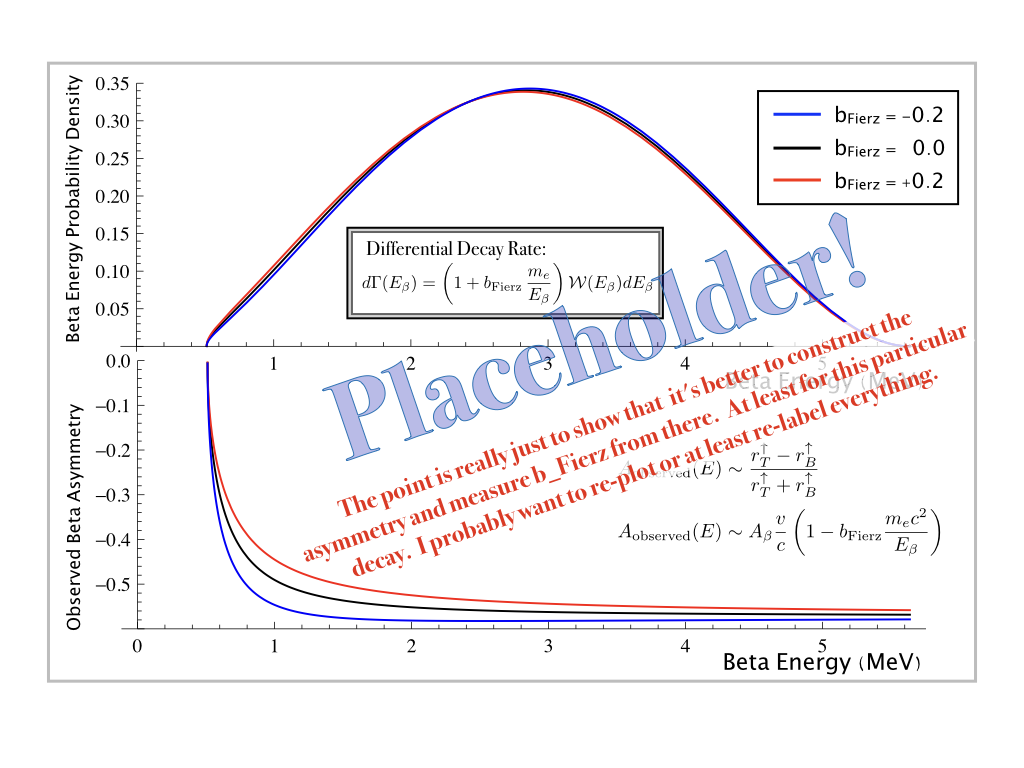
\includegraphics[width=.999\linewidth]
	{Figures/SuperSumSuperRatio_prelim}
	\caption{Here's why it's better to extract $\bFierz$ from an asymmetry, in this case.}	
	\label{fig:supersumsuperratio}
\end{figure}

